\section{Experiments}\label{sec:experiments}
We put into action and assessed the outcomes of pose estimation for both synthetic and real data employing both the fundamental matrix and the trifocal tensor. \footnote{The MATLAB code to reproduce these experiments is available at the GitHub repository: \href{https://github.com/versi379/Two-View-Three-View-Pose-Estimation.git}{https://github.com/versi379/Two-View-Three-View-Pose-Estimation.git}.}

\subsection{Synthetic Data}
We conducted trials on synthetic data to assess pose estimation using both the fundamental matrix and the trifocal tensor across various configurations. The standard experimental setup consists of a collection of spatial points situated within a 400mm-sided cube centered at the world's origin (figura). Points are projected onto three views, and Gaussian noise with a standard deviation of 1 pixel is applied to the image points, unless specified otherwise. A set of 12 points is utilized for computations across various models. The image dimensions are 1800×1200 pixels, representing a sensor size of 36mm×24mm, with a fixed focal length of 50mm. All cameras are aligned to focus on the origin. Results are averaged over 20 simulations of data.\\



\begin{figure}[p]
	\centering
	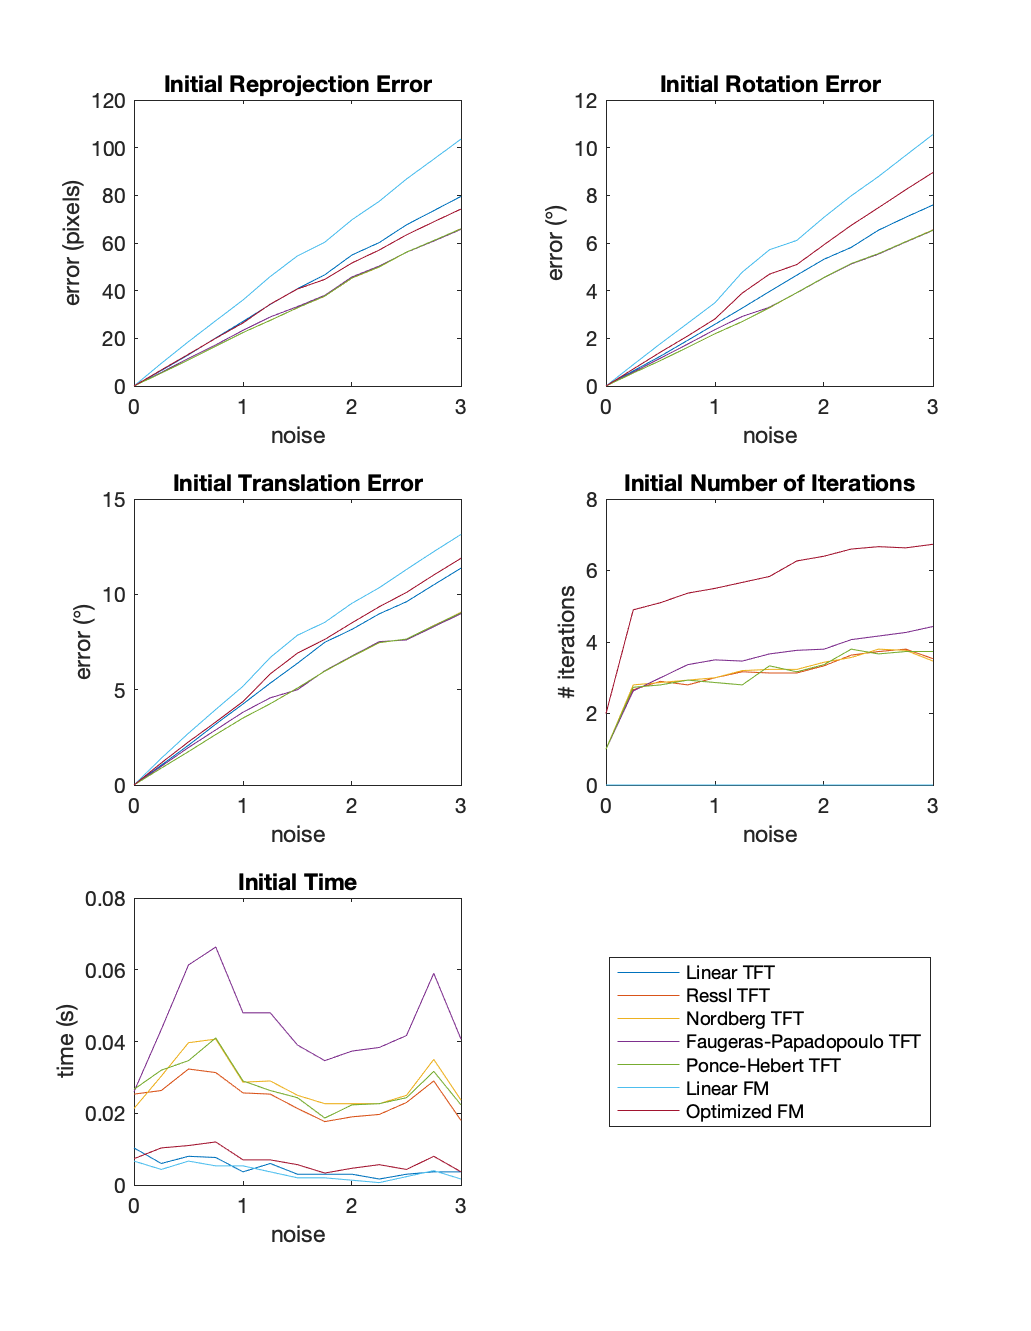
\includegraphics[width=1\textwidth]{Experiments/Synthetic/noise/INITnoisePlots.png}
	\caption{Reprojection error (top-left), rotation error (top-right), translation error (mid-left), number of iterations (mid-right), computational time (bottom-left); when varying the Gaussian noise added to the image points.}
\end{figure}

\begin{figure}[p]
	\centering
	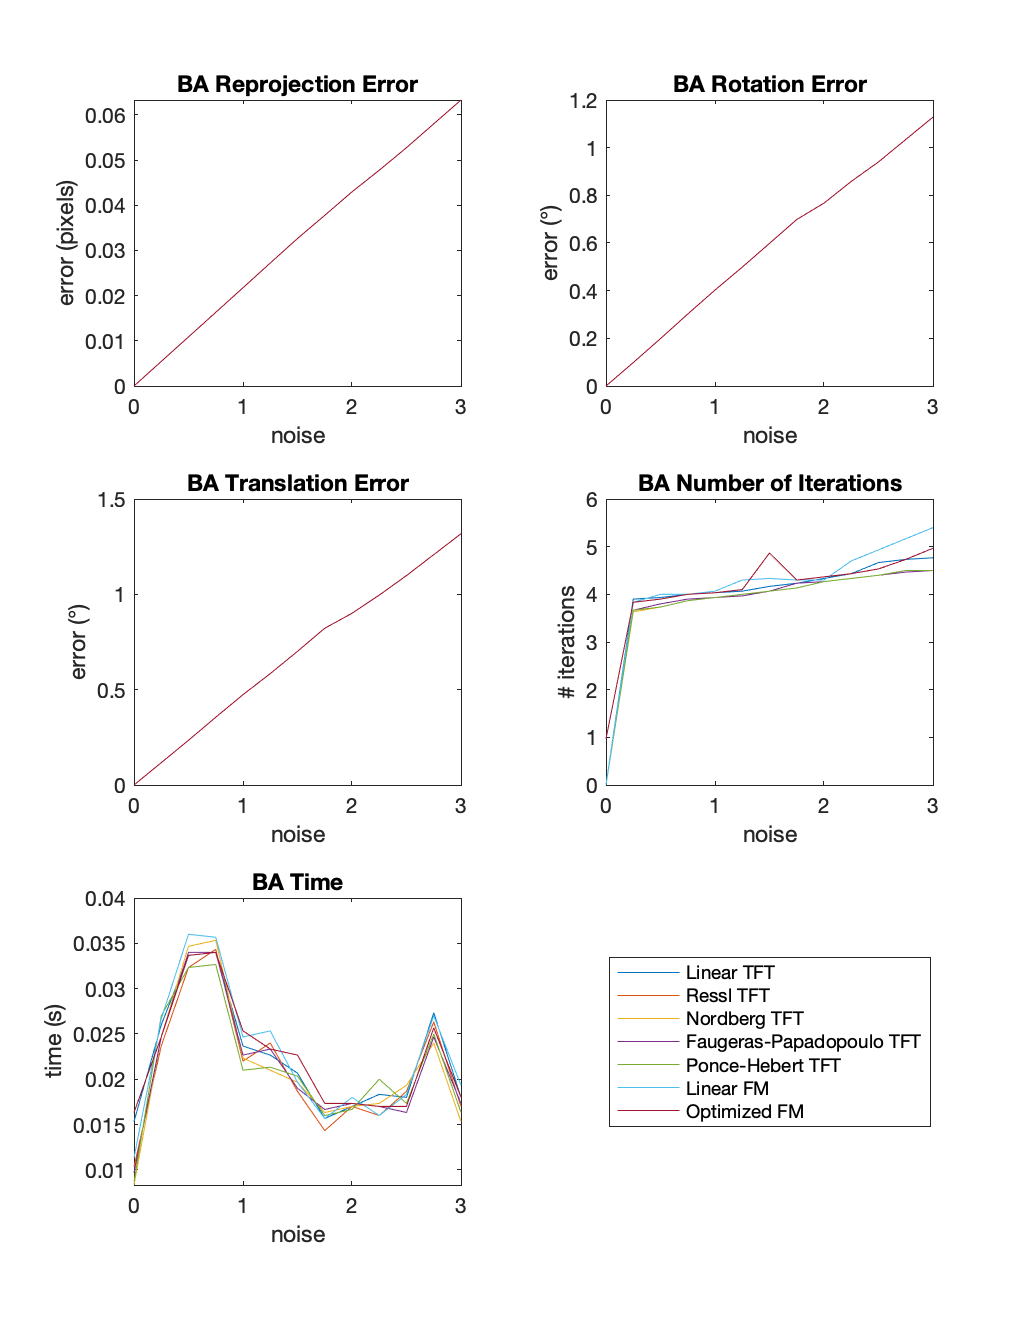
\includegraphics[width=1\textwidth]{Experiments/Synthetic/noise/BAnoisePlots.png}
	\caption{Reprojection error (top-left), rotation error (top-right), translation error (mid-left), number of iterations (mid-right), computational time (bottom-left) after Bundle Adjustment; when varying the Gaussian noise added to the image points.}
\end{figure}

\begin{figure}[p]
	\centering
	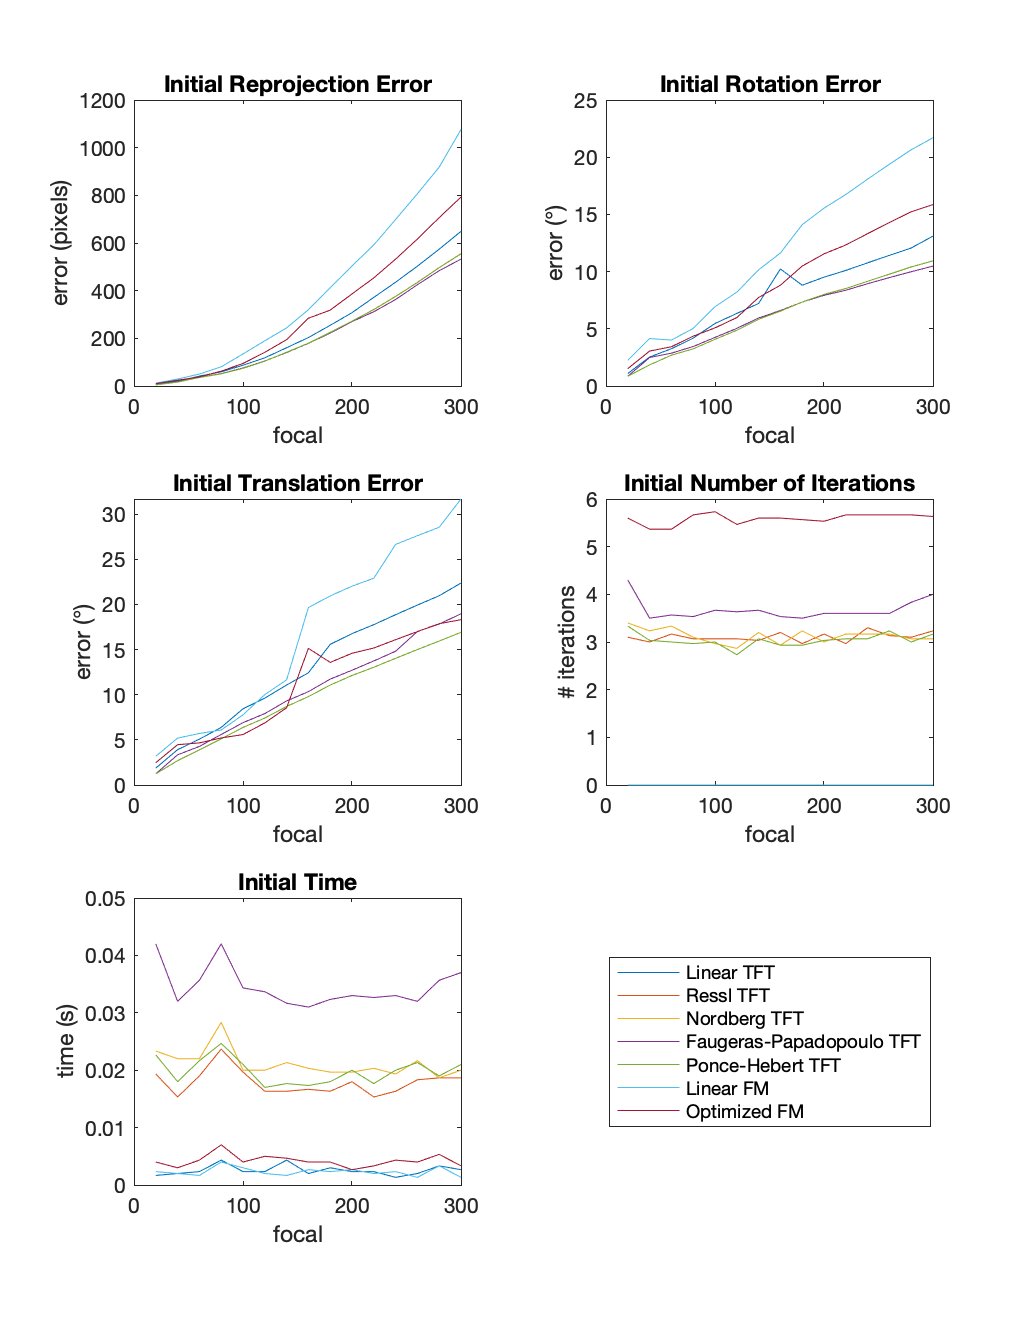
\includegraphics[width=1\textwidth]{Experiments/Synthetic/focal/INITfocalPlots.png}
	\caption{Reprojection error (top-left), rotation error (top-right), translation error (mid-left), number of iterations (mid-right), computational time (bottom-left); when varying the Gaussian noise added to the image points.}
\end{figure}

\begin{figure}[p]
	\centering
	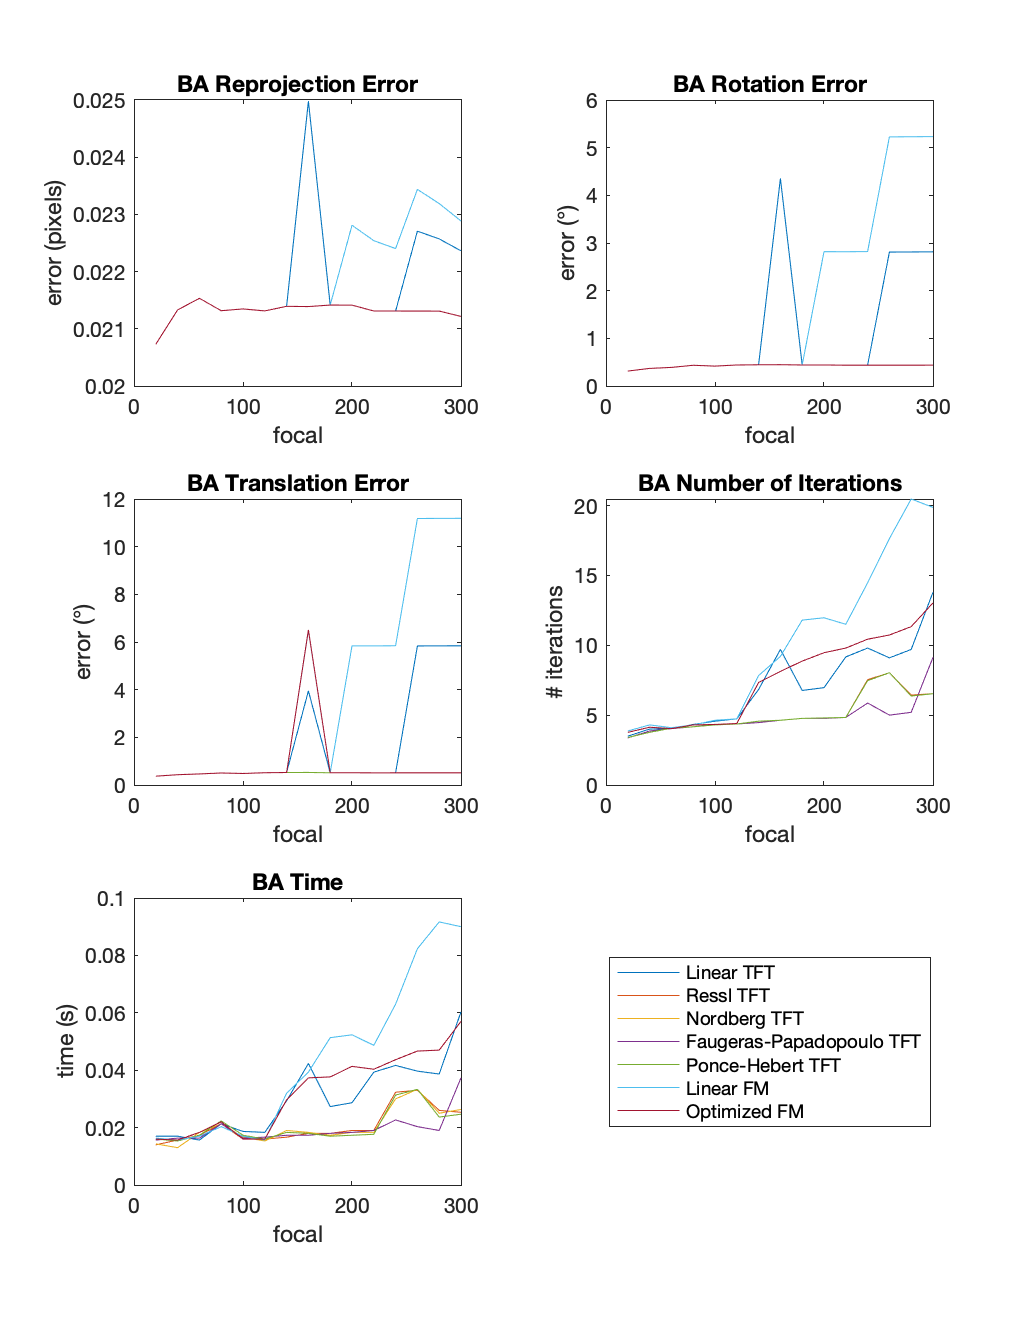
\includegraphics[width=1\textwidth]{Experiments/Synthetic/focal/BAfocalPlots.png}
	\caption{Reprojection error (top-left), rotation error (top-right), translation error (mid-left), number of iterations (mid-right), computational time (bottom-left) after Bundle Adjustment; when varying the Gaussian noise added to the image points.}
\end{figure}

\begin{figure}[p]
	\centering
	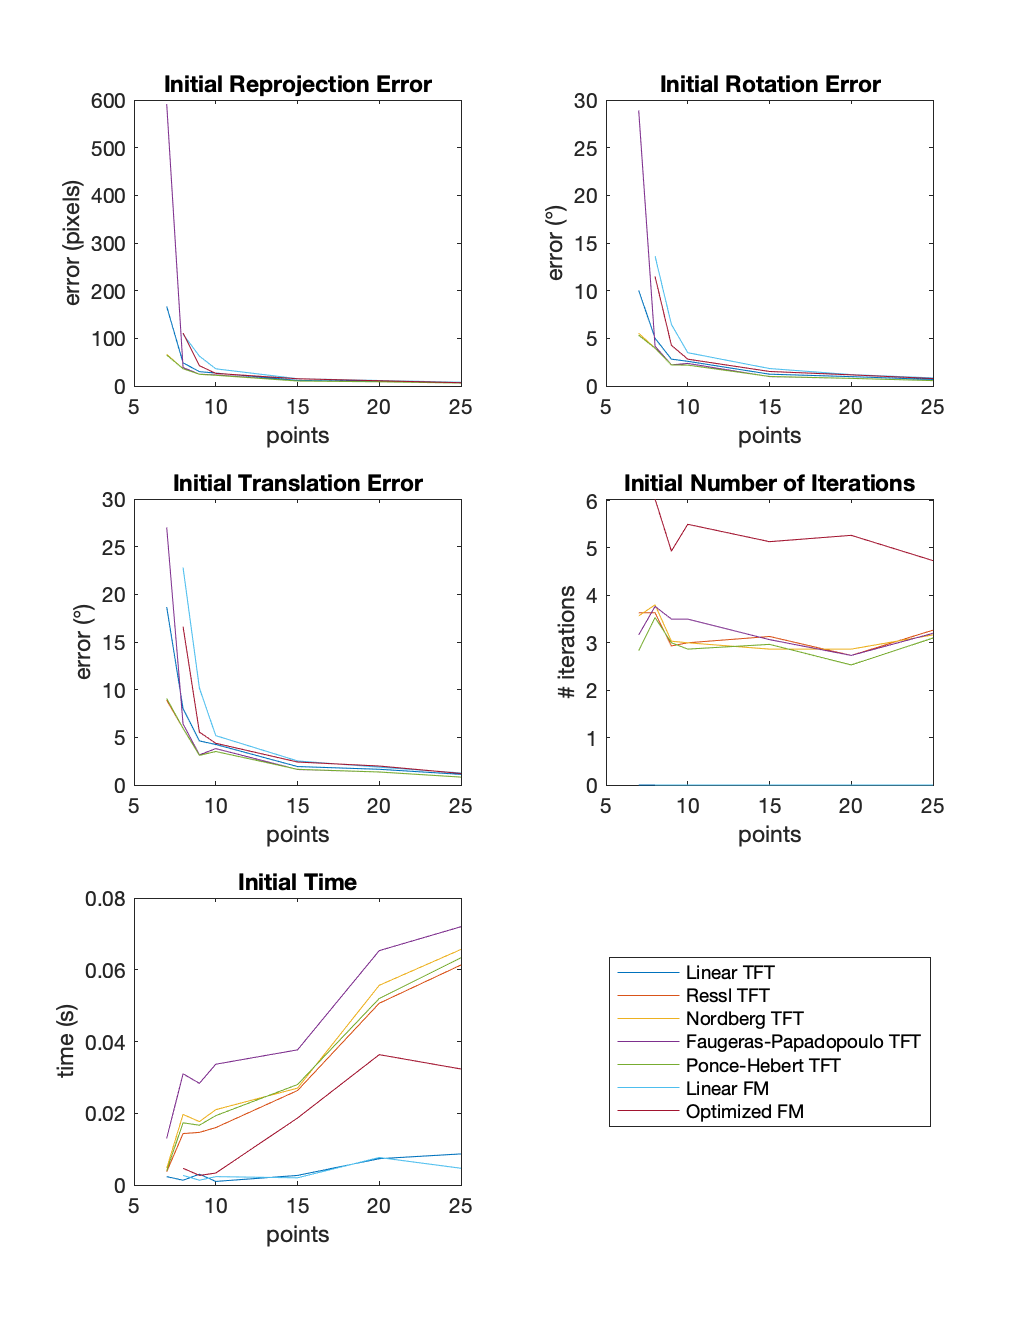
\includegraphics[width=1\textwidth]{Experiments/Synthetic/points/INITpointsPlots.png}
	\caption{Reprojection error (top-left), rotation error (top-right), translation error (mid-left), number of iterations (mid-right), computational time (bottom-left); when varying the Gaussian noise added to the image points.}
\end{figure}

\begin{figure}[p]
	\centering
	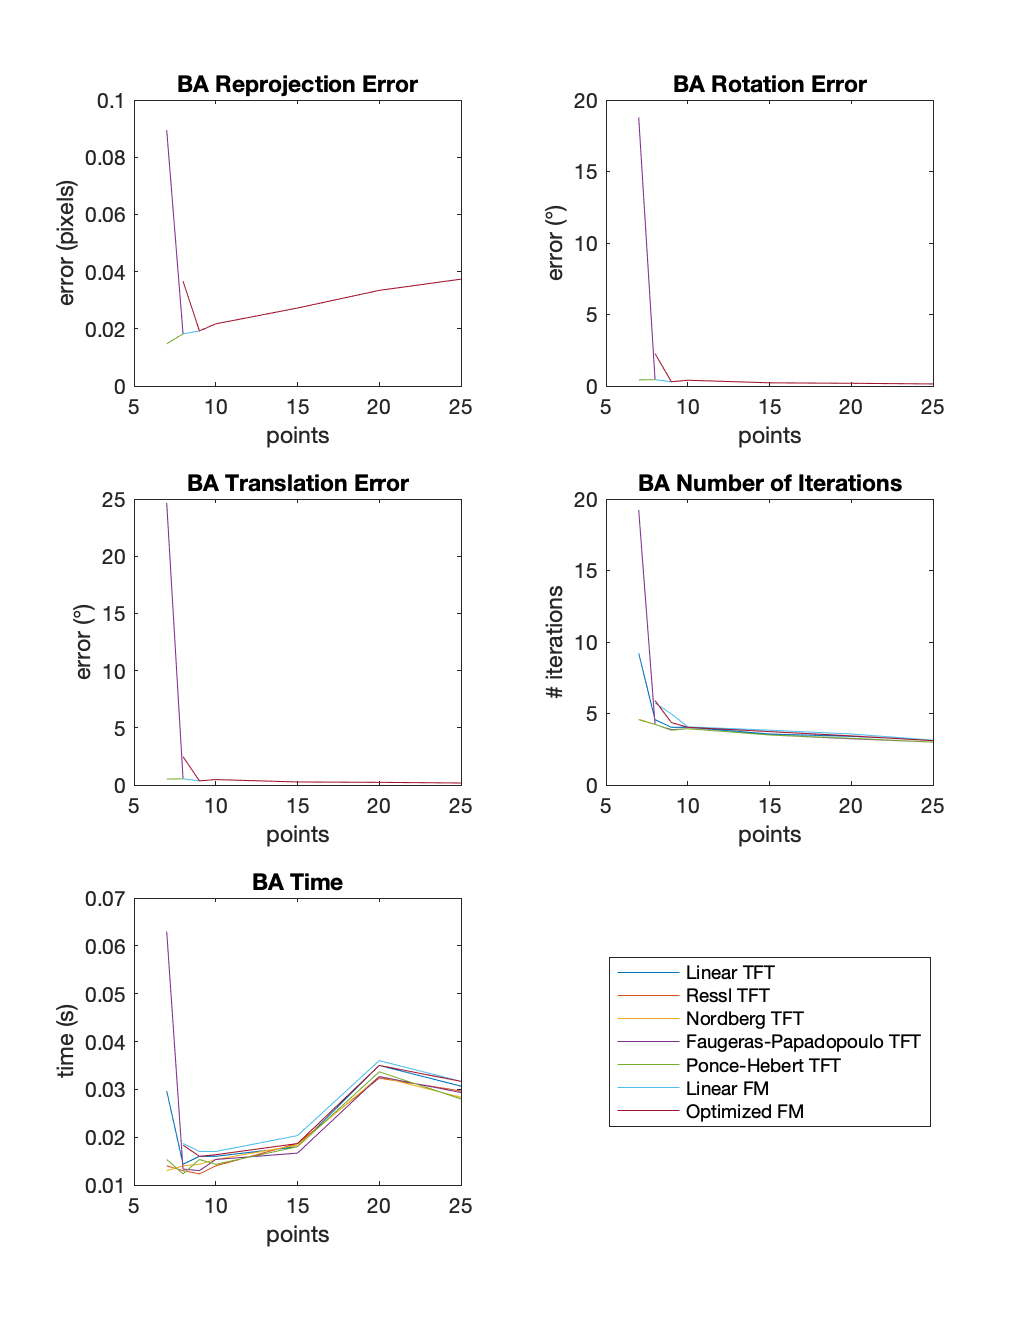
\includegraphics[width=1\textwidth]{Experiments/Synthetic/points/BApointsPlots.png}
	\caption{Reprojection error (top-left), rotation error (top-right), translation error (mid-left), number of iterations (mid-right), computational time (bottom-left) after Bundle Adjustment; when varying the Gaussian noise added to the image points.}
\end{figure}

\begin{figure}[p]
	\centering
	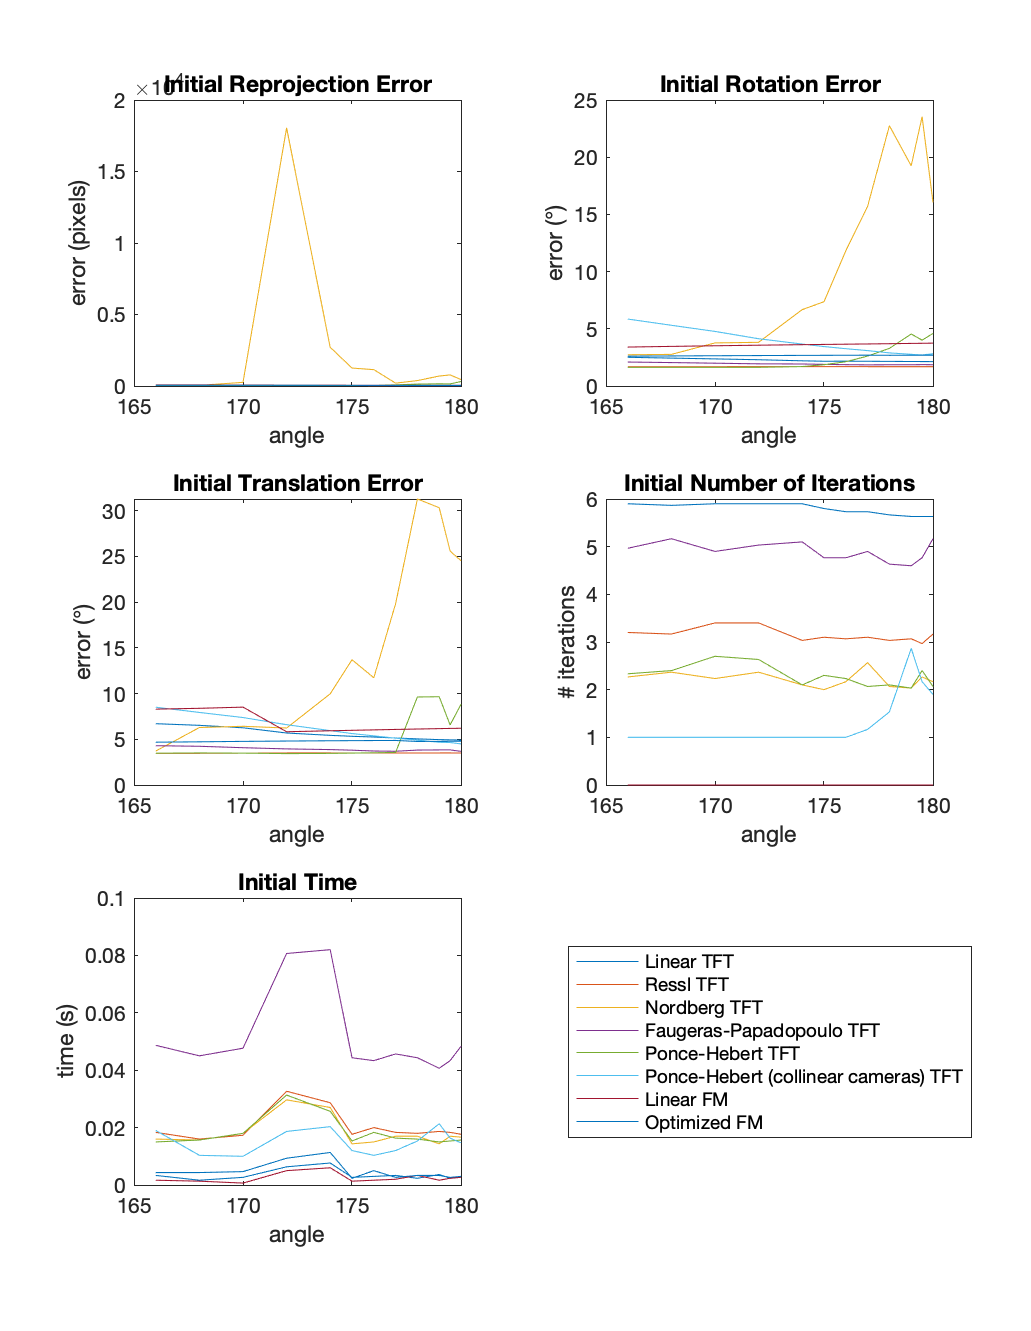
\includegraphics[width=1\textwidth]{Experiments/Synthetic/angle/INITanglePlots.png}
	\caption{Reprojection error (top-left), rotation error (top-right), translation error (mid-left), number of iterations (mid-right), computational time (bottom-left); when varying the Gaussian noise added to the image points.}
\end{figure}

\begin{figure}[p]
	\centering
	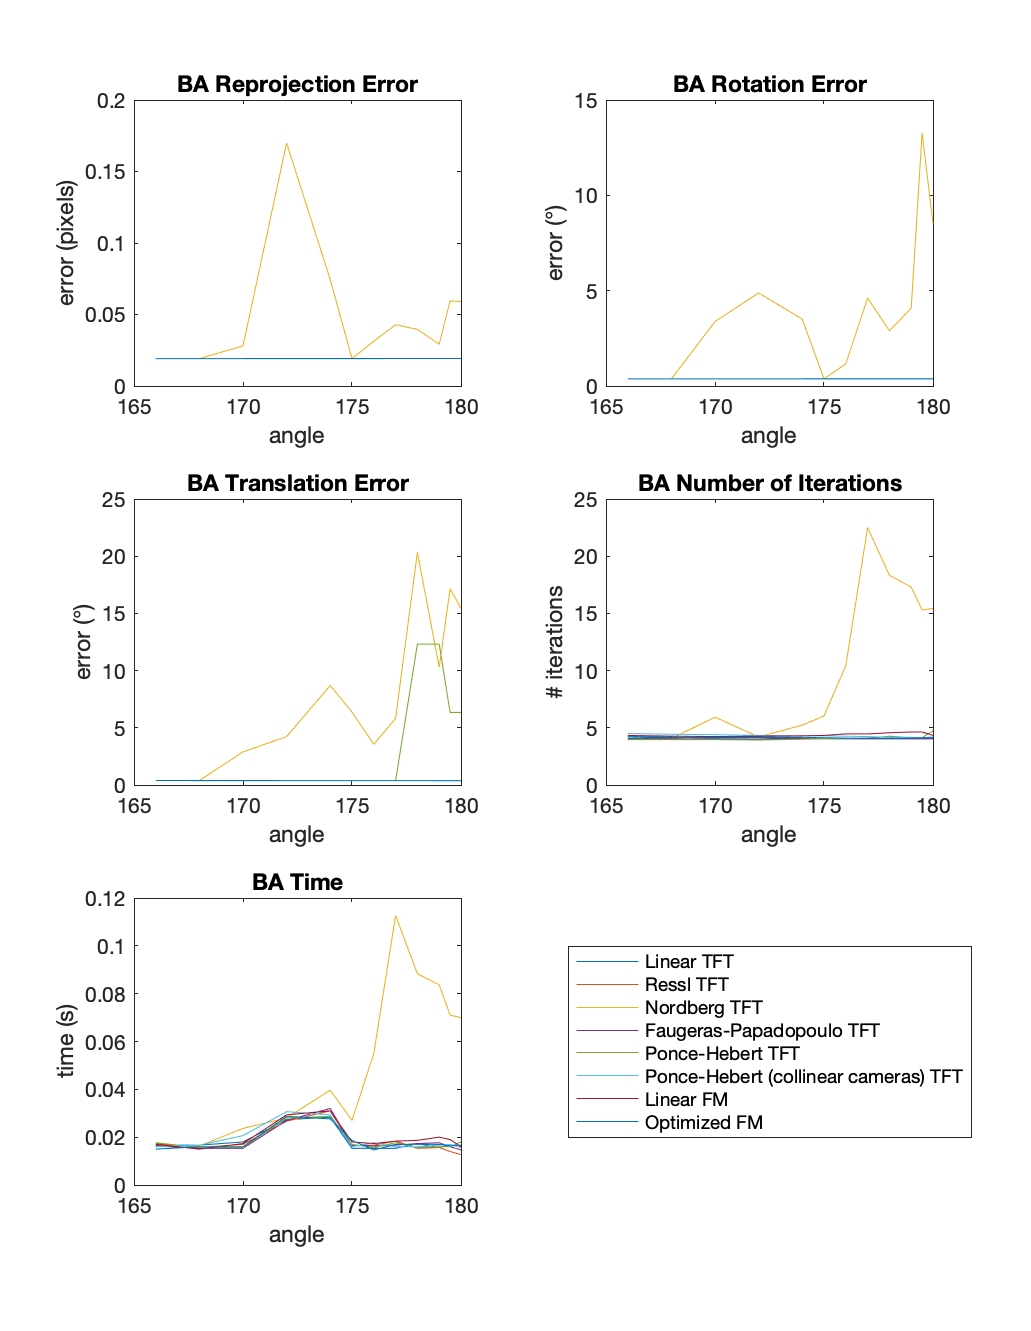
\includegraphics[width=1\textwidth]{Experiments/Synthetic/angle/BAanglePlots.png}
	\caption{Reprojection error (top-left), rotation error (top-right), translation error (mid-left), number of iterations (mid-right), computational time (bottom-left) after Bundle Adjustment; when varying the Gaussian noise added to the image points.}
\end{figure}

\pagebreak

\subsection{Real Data}
In assessing the efficacy of these methods within real-world contexts, we opted to utilize scenes from the EPFL Dense Multi-View Stereo Dataset, presented in \cite{13-epfl-dataset}, provided by the CVLab at EPFL. \footnote{The EPFL Dense Multi-View Stereo Dataset comprising the utilized scenes is available at \href{https://documents.epfl.ch/groups/c/cv/cvlab-unit/www/data/multiview/denseMVS.html}{https://documents.epfl.ch/groups/c/cv/cvlab-unit/www/data/multiview/denseMVS.html}.}\\



\begin{table}[htbp]
  \centering
  \caption{FountainInit}
  \label{tab:fountainInit}
  \begin{tabular}{|*{6}{c}|}
    \hline
     & repr. error (px) & R error ($^{\circ}$) & t error ($^{\circ}$) & \# iter. & time (s)\\
    \hline
    Linear TFT & & & & & \\
    \hline
    Ressl TFT & & & & & \\
    \hline
    Faugeras-Papadopoulo TFT & & & & & \\
    \hline
    Ponce-Hebert TFT & & & & & \\
    \hline
    Linear FM & & & & & \\
    \hline
    Optimized FM & & & & & \\
    \hline
  \end{tabular}
\end{table}

\begin{table}[htbp]
  \centering
  \caption{FountainBA}
  \label{tab:fountainBA}
  \begin{tabular}{|*{6}{c}|}
    \hline
     & repr. error (px) & R error ($^{\circ}$) & t error ($^{\circ}$) & \# iter. & time (s)\\
    \hline
    Linear TFT & & & & & \\
    \hline
    Ressl TFT & & & & & \\
    \hline
    Faugeras-Papadopoulo TFT & & & & & \\
    \hline
    Ponce-Hebert TFT & & & & & \\
    \hline
    Linear FM & & & & & \\
    \hline
    Optimized FM & & & & & \\
    \hline
  \end{tabular}
\end{table}

\begin{table}[htbp]
  \centering
  \caption{HerzJesuInit}
  \label{tab:HerzJesuInit}
  \begin{tabular}{|*{6}{c}|}
    \hline
     & repr. error (px) & R error ($^{\circ}$) & t error ($^{\circ}$) & \# iter. & time (s)\\
    \hline
    Linear TFT & & & & & \\
    \hline
    Ressl TFT & & & & & \\
    \hline
    Faugeras-Papadopoulo TFT & & & & & \\
    \hline
    Ponce-Hebert TFT & & & & & \\
    \hline
    Linear FM & & & & & \\
    \hline
    Optimized FM & & & & & \\
    \hline
  \end{tabular}
\end{table}

\begin{table}[htbp]
  \centering
  \caption{HerzJesuBA}
  \label{tab:HerzJesuBA}
  \begin{tabular}{|*{6}{c}|}
    \hline
     & repr. error (px) & R error ($^{\circ}$) & t error ($^{\circ}$) & \# iter. & time (s)\\
    \hline
    Linear TFT & & & & & \\
    \hline
    Ressl TFT & & & & & \\
    \hline
    Faugeras-Papadopoulo TFT & & & & & \\
    \hline
    Ponce-Hebert TFT & & & & & \\
    \hline
    Linear FM & & & & & \\
    \hline
    Optimized FM & & & & & \\
    \hline
  \end{tabular}
\end{table}
